\documentclass[border=6pt]{standalone}
\usepackage{amsmath}
\usepackage{amssymb}
\usepackage{tikz}
\usepackage{pgfplots}
\pgfplotsset{compat=1.18}
\usetikzlibrary{arrows.meta,calc,positioning}
\begin{document}
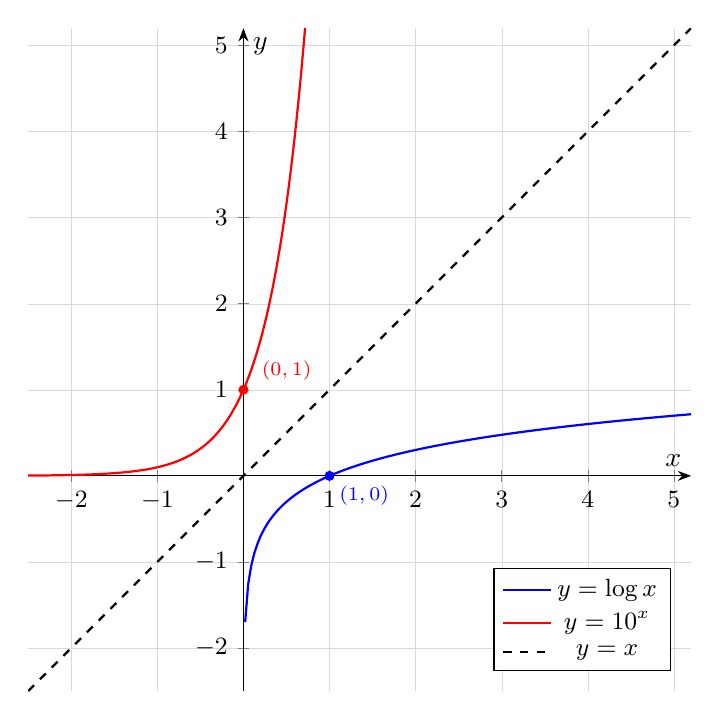
\begin{tikzpicture}
\begin{axis}[
    axis lines = middle,
    xlabel = {$x$}, ylabel = {$y$},
    grid=both,
    grid style={line width=.1pt, draw=gray!30},
    axis line style={-Stealth},
    legend style={font=\small},
    tick label style={font=\small},
    xmin=-2.5, xmax=5.2, ymin=-2.5, ymax=5.2,
    xtick={-2,-1,0,1,2,3,4,5},
    ytick={-2,-1,0,1,2,3,4,5},
    width=10cm, height=10cm,
    legend pos=south east,
]
\addplot[domain=0.02:5.2, samples=150, thick, blue] {ln(x)/ln(10)};
\addlegendentry{$y=\log x$}
\addplot[domain=-2.5:0.72, samples=150, thick, red] {10^x};
\addlegendentry{$y=10^x$}
\addplot[domain=-2.5:5.2, samples=2, thick, black, dashed] {x};
\addlegendentry{$y=x$}
\addplot[only marks, mark=*, mark size=1.6pt, blue] coordinates {(1,0)};
\node[anchor=north west, font=\scriptsize, blue] at (axis cs:1,0) {$(1,0)$};
\addplot[only marks, mark=*, mark size=1.6pt, red] coordinates {(0,1)};
\node[anchor=south west, font=\scriptsize, red] at (axis cs:0.1,1) {$(0,1)$};
\end{axis}
\end{tikzpicture}
\end{document}
